\setchapterpreamble[u]{\margintoc}
\chapter{Summary and Outlook}

%\section{Summary of Results}
\label{sec:summary}

This work presented two oscillation measurements of atmospheric neutrinos using the DeepCore sub-array of the IceCube Neutrino Observatory. Both measurements were based on a newly developed data sample of \num{21914} highly pure track-like events in the energy range between \SI{5}{\giga\electronvolt} and \SI{150}{\giga\electronvolt}. The selection process for these events was described in \refch{data-sample} and consisted of several filtering steps in which background due to detector noise and atmospheric muons was removed. At the final filter level, the contribution of muon background was reduced to $\sim2\%$, the noise background was entirely negligible and the sample consisted almost entirely of neutrino interactions. The zenith angle of each event was reconstructed using a modified chi-square fit to the hit times of the observed light under the simplified assumption that they are well described by the Cherenkov light cone of a minimally ionizing muon. he energy was estimated with a likelihood that takes into account whether or not a sensor in the array has observed light. %While these reconstruction methods are less accurate than more sophisticated methods that were developed more recently, they are also less affected by the precise modelling of the detector properties.
Several quantities produced by the reconstruction algorithms such as the length of the reconstructed track and the goodness-of-fit were fed into a Boosted Decision Tree (BDT) that calculated a particle ID (PID) number for every event that estimates the probability that it originated from a muon neutrino interaction. Both data and simulated pseudo-data were binned in zenith angle, energy, and PID. A minimization algorithm then calculated the best-fit neutrino oscillation parameters by re-weighting the simulated events to match the histograms of the observed data as closely as possible.

\section{Result of the Three-Flavor Oscillation Measurement}
\label{sec:summary-three-flavor}

The first data analysis shown in this work was a measurement of the atmospheric mixing angle and mass splitting in the three-flavor neutrino oscillation model assuming normal mass ordering. This measurement is complementary to oscillation analyses of accelerator neutrinos and the most precise measurement using atmospheric neutrinos to date. The result
\begin{align*}
    \sin^2\theta_{23} &= 0.507_{-0.053}^{+0.050}\\
    \Delta m^2_{32} &= 2.42_{-0.75}^{+0.77} \times10^{-3}\;\mathrm{eV}^2.
\end{align*}
is consistent with previous DeepCore measurements and current global fits.

\section{Result of the Sterile Neutrino Search}
\label{sec:summary-sterile-osc}

The second measurement presented in this work was the search for eV-scale sterile neutrinos. The search was performed under the "3+1" model, where the PNMS matrix is extended by an additional row and column to accomodate the mixing of a fourth neutrino mass eigenstate. The measurement used the same data sample as the three-flavor fit and the same likelihood function calculated in an identical binning. The major technical difference between the analyses was that the neutrino oscillation calculation for the sterile neutrino model was done using a customized version of the \textsc{nuSQuIDS} package. It allowed a computationally efficient way of calculating flavor transition probabilities in the presence of a heavy fourth mass eigenstate that produces a very fast oscillation pattern. The customizations that were developed specifically for this work were the addition of low-pass filters that can analytically produce oscillation probabilities where the contributions due to that heaviest mass eigenstate are averaged out. Another major technical development that separates the sterile neutrino analysis from the three-flavor fit is the introduction of a novel method of incorporating uncertainties in the detector response in a way that is fully decoupled from neutrino oscillation probabilities.

%\subsubsection{Result}
The analysis constrained the $|U_{\mu4}|$ and $|U_{\tau4}|$ elements of the extended PNMS matrix to\todo{extract precise numbers}
\begin{equation}
    \begin{aligned}
        \abs{U_{\mu4}}^2 &< X \\
        \abs{U_{\tau4}}^2 &< Y \\
    \end{aligned}
\end{equation}
at 90\% C.L. while marginalizing over the CP violating phase $\delta_{24}$. This result is valid for both normal ordering and inverted ordering thanks to the approximate degeneracy between the mass ordering and the sign of $\cos(\delta_{24})$. The confidence limits were calculated using Wilks' theorem assuming two degrees of freedom. Spot-checks of the likelihood distributions showed that these limits err on the conservative side. More stringent limits could be obtained by correcting the critical values of the likelihood according to Feldman and Cousins\cite{Feldman_1998}, but the computational expense was deemed too high and the conservative limits sufficient for the purposes of this work. This result is a substantial improvement over the previous DeepCore result and provides the most stringent limit on $\abs{U_{\tau4}}^2$ to date. The constraint on $\abs{U_{\mu4}}^2$ is competitive with other experiments and has the potential to further increase the tension between appearance and disappearance datasets in global fits of the 3+1 sterile neutrino model described in \refsec{global-anomalies}.

\section{Outlook}

The measurement presented in this thesis used only the fraction of the available DeepCore data that could be reconstructed with older reconstruction methods that are optimized for robustness. The purpose of this analysis was not to achieve the highest possible sensitivity, but to verify the integrity of the newly developed data selection techniques and to act as a test bed for newly developed methods of treating uncertainties in the detector properties. Once the tools that were developed for this analysis are combined with more capable reconstruction methods, this new data sample will provide constraints on oscillation parameters that are more stringent than those of any other atmospheric neutrino oscillation measurement and rival the precision of the most recent accelerator experiments.

\subsection{Reconstruction Improvements}
A substantial increase in the sensitivity of both analyses could be achieved by using the table-based reconstruction method described in \cite{lowen-reco-paper}. This algorithm can provide an estimate for the energy and zenith angle for nearly all events passing the Level 5 event filter described in \refsec{data-processing} and has a much higher resolution than the reconstruction method used in this analysis, substantially increasing the statistical power of the analysis. The projected sensitivity that could be achieved with this method is shown in \reffig{retro-sensitivity}.\todo{Compare SANTA sensitivity, add retro sensitivity} With the increased statistical power and resolution also comes a larger burden to accurately model the properties of the neutrino flux, particle interactions and detector properties. The work to bring data and simulation into agreement with the more powerful sample is still ongoing at the time of writing this thesis.
\begin{figure}
    \centering
    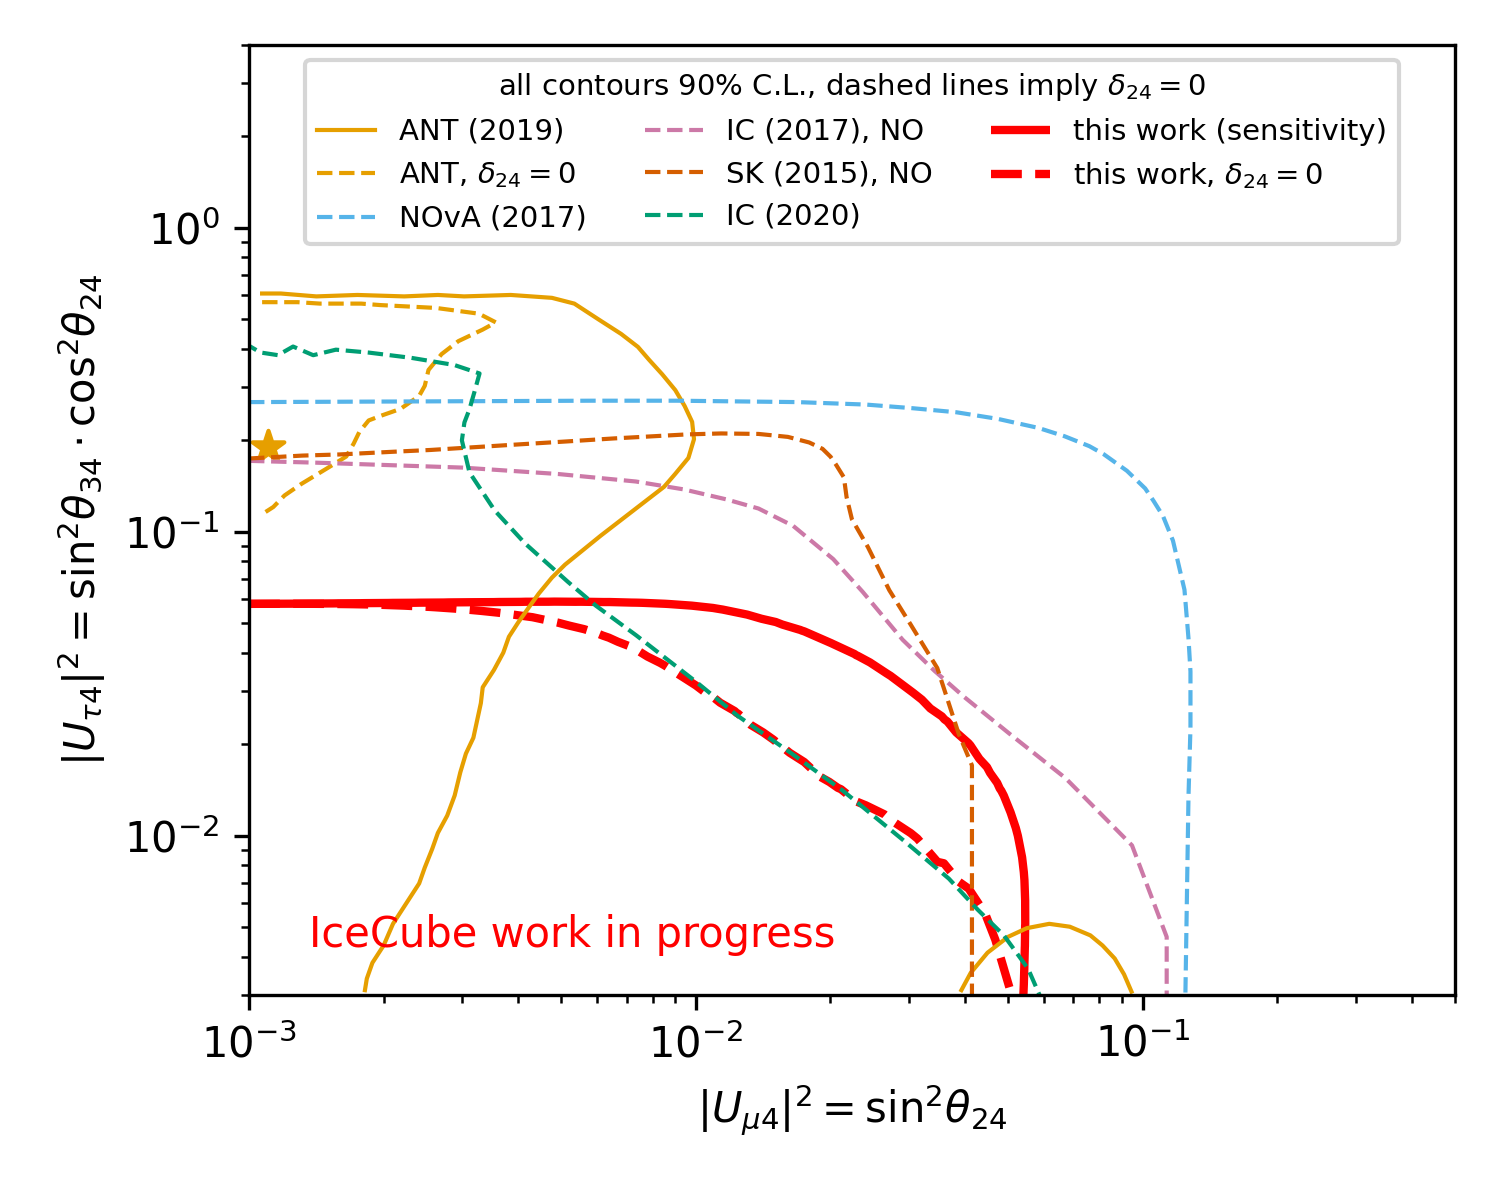
\includegraphics[width=0.7\linewidth]{figures/summary/Sterile_mixing_sensitivity_90pct_retro.png}
    \caption{Projected sensitivity of the sterile neutrino search when using the table-based reconstruction method.\label{fig:retro-sensitivity}}
\end{figure}

\subsection{Ice model}
The major distinction of the IceCube Neutrino Observatory compared to most other neutrino detectors is that the detection medium is the naturally occurring ice at the South Pole, rather than an artificially produced material. The ice consists of many layers with different optical qualities that are the result of varying snow depositions over the last \num{100000} years. Understanding the precise properties of the ice at every position in the detector requires complex calibration procedures that are beyond the scope of this work. Recently, calibration efforts at IceCube have led to a new ice model that takes into account the birefringent scattering of light at the boundary of ice crystals that is currently under review for publication\sidecite{tc-2022-174}. The birefringence bends light rays into the direction of the flow of the glacier, which affects the zenith angle reconstruction for events in DeepCore in particular. Future iterations of DeepCore oscillation studies are expected to include this new ice model in order to achieve a better agreement between data and simulation.

\subsection{Treatment of systematic uncertainties}
\subsubsection{Detector uncertainties}
In order to perform the sterile oscillation search, a novel method of interpolating between different MC sets has been developed that allows re-weighting individual events based on changes in the detector response. The need for this development arose from the discovery that the effect of a change in detector properties in each bin of the analysis is coupled to the values of the neutrino oscillation parameters. In the three-flavor analysis, this problem was addressed by interpolating the gradients of the bin counts with respect to detector parameters over a grid of points in the mass splitting parameter $\Delta m^2_{31}$ as described in \refsec{hypersurfaces}. For the sterile analysis, however, the dimensionality of the grid needed to cover all oscillation parameters made this approach unfeasible. The new method, described in \refsec{ultrasurfaces}, completely decouples the detector response from oscillation parameters and thereby eliminates the need for any interpolation. This property makes it universally applicable to any oscillation study probing arbitrarily complex oscillation phenomena. In addition, the method opens the door to using unbinned likelihood functions in future analyses, which was impossible in the past because previous methods such as the one described in \sidecite{multisim} are inherently binned. In the near future, this new method of calculating event-wise weights based on posterior estimates will be expanded upon and has the potential to become the new standard treatment for detector uncertainties for neutrino telescopes.

\subsubsection{Atmospheric flux}
The treatment of atmospheric neutrino flux uncertainties used in this work is based on the Barr blocks method that was published in 2006\cite{Barr2006}. Since then, new methods of modeling variations of the atmospheric flux have been developed that decrease the overall relative uncertainty by up to 40\% and also provide a data-driven parametrization of the flux variations\sidecite{Fedynitch_2022}. Incorporating these developments into the oscillation data analysis has the potential to improve the agreement between data and simulation and to increase the sensitivity.

\subsection{IceCube Upgrade}
The IceCube Collaboration is planning to deploy seven strings of densely spaced optical sensors within the DeepCore fiducial volume in the near future that will form the \emph{IceCube Upgrade}\sidecite{icecube_upgrade}. The Upgrade will not only be instrumented more densely than the existing DeepCore array, but will also contain new types of optical sensors that contain multiple PMTs. This will increase the total photocathode area and add the ability to differentiate the arrival direction of light on each sensor. The new array is expected to lower the energy threshold for the detection of atmospheric neutrinos to $\sim\SI{1}{\giga\electronvolt}$. The Upgrade strings will also incorporate several calibration devices that will further improve the modeling of the ice and detector properties. The sensitivity of the Upgrade array to neutrino oscillation parameters is expected to greatly improve over that of DeepCore as shown in \reffig{upgrade-sensitivity} for the atmospheric mass splitting and mixing angle.
\begin{figure}
    \centering
    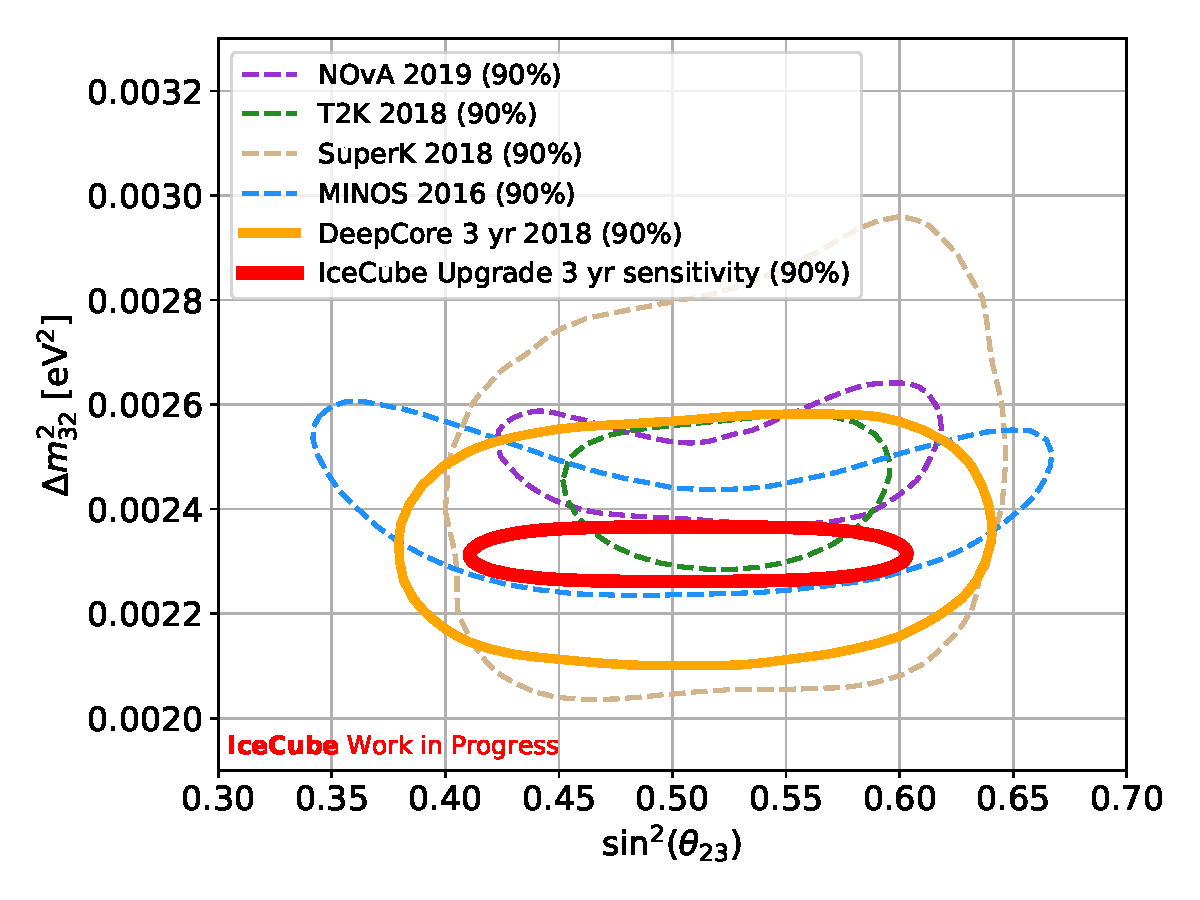
\includegraphics[width=0.7\linewidth]{figures/summary/June26_Upgrade_NuMu_Disappearance_Sensitivity.pdf}
    \caption{Expected sensitivity to the atmospheric neutrino oscillation parameters with three years of Upgrade data compared to recent results from DeepCore and other experiments. Figure taken from \cite{icecube_upgrade}.\label{fig:upgrade-sensitivity}}
\end{figure}


\chapter{Conclusion}

This work presented the first results to be obtained using a newly developed eight-year data sample of IceCube's DeepCore sub-array. This sample is the result of an effort by the IceCube Collaboration over several years to improve the detector calibration and selection process to achieve a better agreement between data and simulation. The events used for the measurement in this work were reconstructed using a simple and fast geometric algorithm that only reconstructs the direction for very clean, track-like events. With this  sample of high-quality DeepCore events, the analysis was able to achieve a good fit to the data and to produce a measurement of the standard atmospheric neutrino oscillation parameters $\theta_{23}$ and $\Delta m^2_{32}$, as well as constraints on sterile neutrino mixing that are the best in its class of experiments. The work on this sub-sample also led to important developments of analysis tools and techniques that are directly applicable to studies with higher statistics and more modern reconstruction methods. These developments include the invention of a novel method of interpolating between different Monte Carlo sets in a way that is decoupled from neutrino oscillation effects, and several filtering techniques to efficiently calculate neutrino oscillation probabilities in the presence of heavy neutrino states.

Neutrino oscillations are the first clear evidence of physics beyond the Standard Model. Neutrinos must have non-zero masses for the phenomenon to occur, but it is unclear how large those masses are and how they acquire these masses in the first place. The data analysis presented in this work probed the oscillation pattern of neutrinos that are produced in the atmosphere of the Earth for signs of heavy neutrino mass eigenstates that do not interact with the Weak force. These additional mass eigenstates could be a byproduct of the process that generates neutrino masses and might explain the smallness of the masses of the active neutrino flavors. The search for these states presented in this work was made by probing the $\nu_\mu$ disappearance probability under the assumption of the minimal "3+1" model with one additional mass splitting between of $\order{\SI{1}{\electronvolt\squared}}$. The particular choice of mass splitting was based on experimental anomalies that have been found in some accelerator experiments and measurements of the neutrino flux originating in radioactive decay. The null-result of the search presented in this work further increases the tension between the anomalies observed in the $\nu_e$ appearance channel probed in LSND and MiniBooNE and the constraints from $\nu_e$ and $\nu_\mu$ disappearance datasets. Given that his tension was already approaching the $5\sigma$ threshold in global fits, it is unlikely that the simple "3+1" model of sterile neutrino oscillation can explain the anomalies that initially motivated the measurement performed in this thesis. Using the data selection and analysis methods that have been developed during the work that led to this thesis, DeepCore measurements with a greatly increased statistical power will be able to probe neutrino oscillations for signals of a rich landscape of other possible phenomena beyond the Standard Model.
